\documentclass[12pt,twoside,a4paper]{article}
\usepackage{titlesec}
\usepackage{chngcntr}
\usepackage{float}
\counterwithin{figure}{section}
\counterwithin{figure}{subsection}
\usepackage[margin=25mm]{geometry}
\linespread{1}
\titleformat*{\section}{\fontsize{14pt}{2}\bfseries}
\titleformat*{\subsection}{\fontsize{13pt}{2}\bfseries}
\titleformat*{\subsubsection}{\fontsize{13pt}{2}\bfseries}
\usepackage[T1]{fontenc}
\usepackage{listings}
\lstset{
    breaklines=true,
}
\usepackage{mathptmx}
\usepackage{graphicx}
\usepackage{enumitem}
\usepackage[utf8]{inputenc}
\usepackage[english, polish]{babel}
\usepackage[T1]{fontenc}
\graphicspath{ {imgs/} }

\begin{document}
\selectlanguage{polish}
\begin{abstract}

Simple object state detection using camera image / 

W poniższej pracy przedstawiono proces projektowania i tworzenia systemu, który identyfikuje stan obiektów przy użyć obrazu z kamery. Obiekty stanowią partie rozbitych jaj kurzych, które przypisywane są do jednej z dwóch poniższych klas:
\begin{enumerate}
\item nieuszkodzone żółtka jaj otoczone białkiem jajecznym albo czysta linia produkcyjna
\item uszkodzone żółtka albo nieuszkodzone żółtka otoczone szczątkami uszkodzonych żółtek
\end{enumerate}

Na początku opisano proces rozbijania jaj, oraz oddzielania białka od żółtka. Następnie przeanalizowano rynkowy popyt na system automatyzujący ten proces.
Przeprowadzono badania jakościowe istniejących rozwiązań dla tego problemu, oraz usprawnień, jakie można w nich dokonać.
Podjęto decyzję o zaprojektowaniu i wykonaniu protoypu systemu, który montowany będzie na maszynach rozbijających jaja firmy OVO-TECH.
Omówiono konstrucję tego systemu, algorytmy, jakie są w nim zaimplementowane, a następnie wykonano i przetestowano prototyp.
Autor poniższej pracy przewiduje, że wykonany system zastosowanie w firmach farmaceutycznych produkujących leki z białka jajecznego, w cukierniach, które potrzebują oddzielania białek od żółtek do procesów piekarniczych takich jak ubijanie piany z białek, oraz w firmach produkujących odżywki dla sportowców.



\end{abstract}

\selectlanguage{english}
\begin{abstract}
The scope of this work is process of creating a device that automatically assigns broken eggs into one of two following classes:
\begin{enumerate}
\item intact yolks surrounded with egg white or clear processing plant line
\item damaged yolk or intact yolk surrounded with damaged yolk parts
\end{enumerate}
The implementation of such device is preceded with research that compares various methods of recognizing the camera image, taking into account their performance in terms of computation resources, and in terms of correctness of the recognition.
The working prototype is successfully developed and tested.
The device will be mass produced as a module of OVO-TECH rz-1 egg braking machine, to improve machine usefulness for following recipients:
\begin{enumerate}
\item Pharmaceutical companies that manufacture medicines out of egg-white and require high standards in terms of egg-white cleanness
\item Confectioneries that require clean egg white for baking procedures, such us egg foaming process
\item Athletes nutrition producers
\end{enumerate}


\end{abstract}

\tableofcontents


\section{Introduction}
\subsection{Industrial egg processing}
In a following thesis an industrial problem - chicken egg white and yolk separation - is analysed in terms of possible automation and improvements in currently used techniques.

Chicken egg is a widely used ingredient of food, athletes nutrition and medicines. Simplified structure of chicken egg is commonly known: prior to processing and using the egg, its shell has to be removed first, what is done in cracking process. It is estimated that 1.8 trillion chicken eggs are used yearly around the world\cite{trillion}, and most of them are consumed without their shells. 

\begin{figure}[H]
\centering
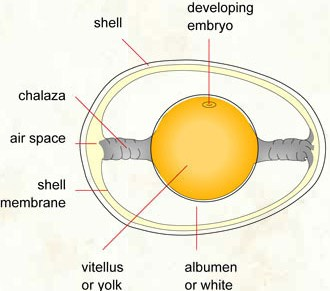
\includegraphics[width=0.4\paperwidth]{structure}
\caption{chicken egg structure, Src: www.gardening-for-wildlife.com}
\end{figure}


\begin{figure}[H]
\centering
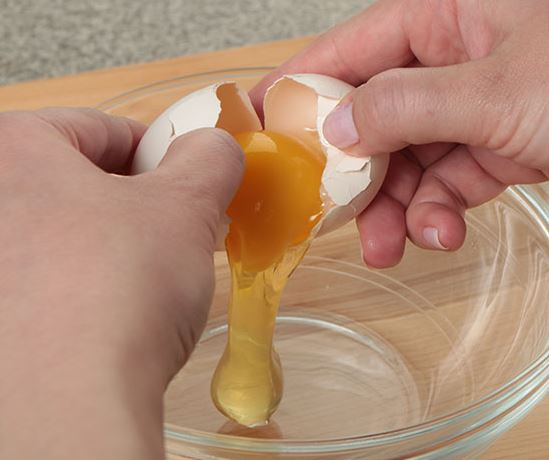
\includegraphics[width=0.4\paperwidth]{crack}
\caption{Manual egg cracking, Src: www.media.eggs.ca}
\end{figure}

For many companies, raw eggs are required to be not only removed from shells, but also egg-yolk and egg white has to be separated.
This is due to following applications:


\begin{itemize}
\item Confectioneries and bakeries utilize egg white foam as an ingredient for their products.
Egg white foam is obtained by aeration (also known as beating / foaming / whipping) process.
Comprehensive process description was provided by one of the bakers:

"When air is incorporated into a liquid or viscous solution, the solution entraps the air bubbles, forming a foam. If the foam is stabilized by proteins, it leavens a food, increasing its height and reducing its density. The viscosity of all egg products is ideal for incorporating air cells during the whipping or beating process. As whipping or beating progresses, air bubbles decrease in size and increase in number, all the time surrounded by egg proteins. Liquid egg products have low air-liquid interfacial tension; thus, when eggs are beaten or whipped, the proteins denature, or simply, they unfold. This exposes two oppositely charged ends of the protein molecule: the hydrophobic, or water-hating end, and the hydrophilic, or water-loving ends. The proteins align themselves between the air and water, securing the air bubbles with their hydrophilic chains pointing into the water and dangling their hydrophobic chains in the air. During baking, these proteins bond with each other, forming a delicate, yet reinforced network.

Egg whites do this much better than yolks because of the unique proteins found in whites. In fact, even though the term foam technically refers to any system where there are entrapped air bubbles, in the food industry, when discussing egg white products, the term tends to be exclusive to egg whites foams. This is because egg whites, unlike any other natural food ingredient, are able to create the largest possible food foam, a foam six to eight times greater in volume than unwhipped, non-aerated liquid egg white

Whole eggs and egg yolks can also increase the volume of foods, including certain baked goods and dairy desserts such as ice cream and custard, but just not as much as egg whites alone. Visually, whipped yolks may double or triple in volume, while whipped whole eggs produce less volume than either yolks or whites whipped separately. They are also less thick than yolks alone." \cite{eggprop}
\item Biotechnology companies make attempts to manufacture medicines for rare diseases from egg white. This is new and emerging branch of pharmaceutical industry, yet very promissing. For example, Synageva Biopharma that their life-saving proteine from egg whites was recently (February 2015) acquired by Alexion for \$8.4 billion.
\item Athletes nutrition producers produces their powders and tabs that are supposed to accelerate muscle growth from egg whites, while yolks are often treated as waste
\item Dried egg powder that is used to extend egg edibility time is also often product separately from egg white and egg yolk.

\end{itemize}
All those facts lead to conclusion, that there exist a large market and potential demand for solutions that would crack the egg and separate egg whites from egg yolks in an automatic way.

Author of this thesis managed to find four companies that already produce machines addressing such problem:
\begin{itemize}
\item Egg King, located in USA
\item Ovobel in Belgium
\item Sanovo from Denmark
\item Ovo-tech from Poland
\end{itemize}
Ovo-tech company was contacted by author and enquired about the way that RZ-1 machine that they product operates. 
It appeared, that during last 4 years multiple attempts were made by this company to separate whites from yolks of freshly broken eggs in a mechanic way. 
Obtained solutions (RZ-1 separation module) proved to be working good enough for some companies, while other rejected them as imperfect and declared intention to buy devices in the future, provided that adequate improvements will be made.
UWAGA tutaj napisz jednym zdaniem po środku, że czasem rozdzielenie jest niedostatecnzie dokładnie.

Nine companies were inquired whether or not would they invest in improved Ovo-tech machine, provided that egg white will be visually clean of yolk parts.
Eight of them replied positively that they would seriously consider such offer since their processing plants would benefit in terms of product quality or manpower cost on such improvement.

One of these companies purchased some ovo-tech machines, but is nevertheless displeased with their separation ratio.
This company currently is undergoing a procedure of obtaining US Food Drug Administration (FDA) approval for wide distribution of their egg-based medicine.
Executives of this client suspect that using machines with better egg separation will increase their chance for positive outcome of above process.

\begin{figure}[H]
\centering
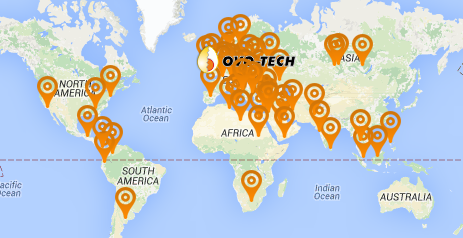
\includegraphics[width=0.4\paperwidth]{map}
\caption{Ovo-tech egg braking machines operating over the world}
\end{figure}


\subsection{Problem formulation}
Ovo-tech observed that a simple dependence exists: the older the egg is, the more likely its yolk is degenerated inside the egg shell. Also, if an egg processed by RZ-1 machine is old or the chicken was feed improperly the yolk might might break during the cracking phase.
Also, a yolk damage is possible due to cracker imperfections such us being calibrated for different size or weight eggs.

A mixture of damaged yolk and white is created in a result of processing a bad quality egg (old and/or damaged), and it is not possible to properly separate it into two initial components using the rz-1 separation module.
Eliminating the batches containing fuzzy yolk should decrease chances of accidentally processing the contaminated eggs, while the risk of egg contamination generally increases with egg age.

Ovo-tech deals with those cases by encouraging companies to hire a person that manually removes the eggs from an accumulating batch (See 2.1 subchapter), but is not satisfied in cost that is additionally generated by this solution.
\begin{figure}[H]
\centering
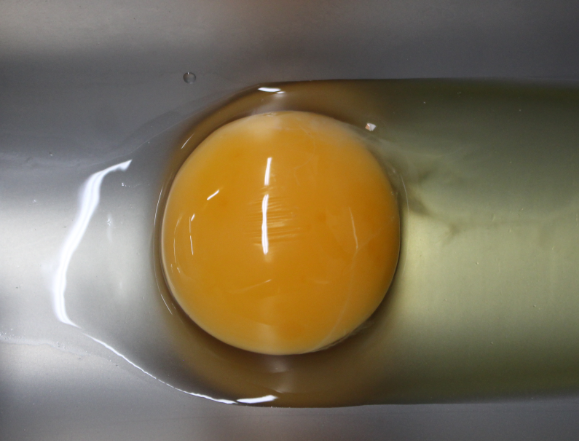
\includegraphics[width=0.4\paperwidth]{prop}
\caption{Properly cracked egg}
\end{figure} 

 
\begin{figure}[H]
\centering
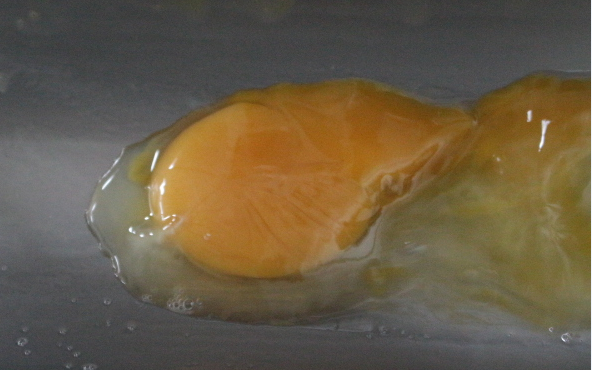
\includegraphics[width=0.4\paperwidth]{damg}
\caption{Damaged yolk in improperly cracked egg}
\end{figure}

UWAGA tutaj dłuższe zdanie na temat, że przeanalizowawszy powyższe kwestie sformuowano project goals jako:
Thus, project goals are formulated as:
\begin{enumerate}
\item Finding an effective method for automatically detecting yolk-and white mixture state.
\item Implementing such method in a prototype device that utilises the discovered method.
\end{enumerate}


\section{Problem analysis}
\subsection{Host machine}
UWAGA tu dwa - trzy zdania więcej, że dobrym metoda pokazania będzi ta maszyna
The machine that will be extended with the module prototype prepared in this thesis is OVO-TECH RZ-1 model.

\begin{figure}[H]+
\centering
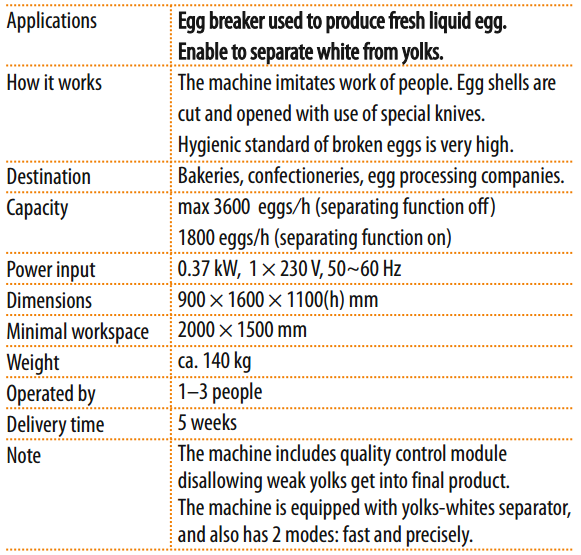
\includegraphics[width=0.4\paperwidth]{rz1table}
\caption{Rz-1 unit basic parameters}
\end{figure}


\begin{figure}[H]
\centering
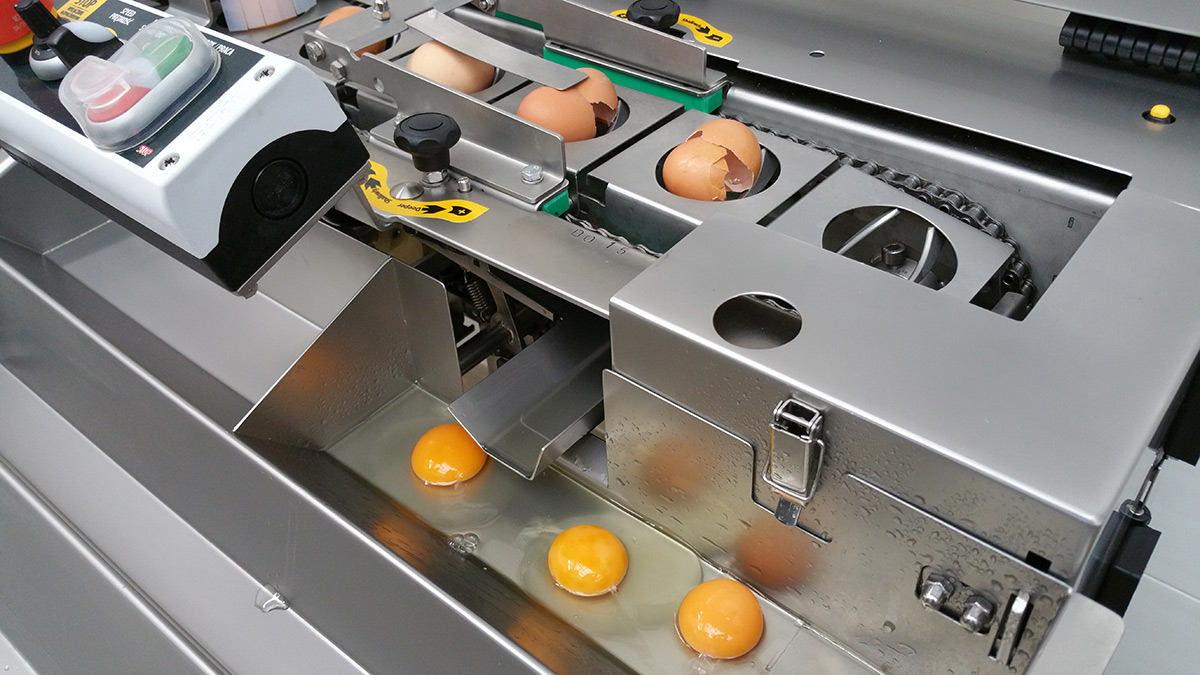
\includegraphics[width=0.4\paperwidth]{rz1crack}
\caption{Egg cracking  module of RZ-1 unit}
\end{figure}


The RZ-1 machine operates in a following way: UWAGA see figure no blablabla
\begin{enumerate}
\item Eggs are directed into one-line flow, and mechanically aligned

\item Cracking module cuts the incoming egg surface from below with two knives that are aligned in direction of egg focal radius.
\item The knives imitate human hands work by opening the previously notched egg.
\item The cracked eggs are accumulated in a movable utensil for optical assessment. 
If the egg yolk appears to be broken, it is removed by an operator from the processing plant.
\item Cracked eggs are transported by sliding to white and yolk separating module.
\item Separation  is done in a mechanic way while eggs slide over specificly shaped gap that only egg white fills in, while the egg yolks remain intact.
\end{enumerate}

\begin{figure}[H]
\centering
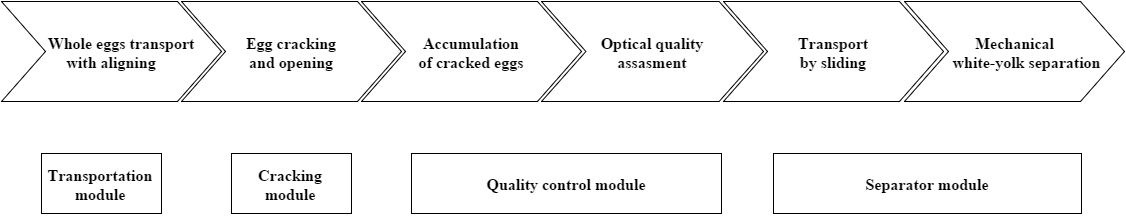
\includegraphics[width=0.8\paperwidth]{process}
\caption{RZ-1 Egg processing  - process and plant structure}

\end{figure}
RZ-1 operates in two modes:
\begin{itemize}
\item Precision mode
\item Fast mode
\end{itemize}
UWAGA że fast mode nie jest rozważany przeze mnie
Precision mode is used widely with bad quality eggs to extend amount of time for optical assessment in (5) phase.

UWAGA tutaj ciut więcej, że te a te processy są automatyczne, a te i te są nieautomatyczne; automatise zamiast replace
The authors idea is to replace the whole Quality Control module with custom designed module, that will automatically asses broken egg quality and remove them mechanically.
The creation of the mechanical element is out of the scope of this work and is handled by Ovo-tech engineers.
The egg accumulation will not longer be required, as well as the work of qualified expert that optically assased the egg quality is not needed any more.



More advanced OVO-TECH models such us RZ-3, RZ-6 and RZ-8 will be also considered for further research.


\subsection{Establishing framework for product cleanness assessment}

The requirement is to create a system able to detect all product batches containing badly-cracked eggs.
A batch is defined as a mixture of freshly broken eggs containing egg yolks, egg white, not containing the egg shells, that is present on a the sliding slope that transports the product to separating module.

UWAGA uciekło zdanie

After request for clarification, client made 60+ pictures of product during machine operation and classified them manually, thus requirement is less ambiguous.


Client decided that batch intact egg yolks should be removed from processing line if:

\begin{enumerate}
\item intact yolk is surrounded by homogeneous mixture of another damaged yolk and white.
This is the most strict (in terms of cleanness) case, that generates less strict cases:
\item intact yolk surrounded by damaged yolk blobs
\item fuzzy (damaged) yolk that still keeps its shape without mixing with white
\item damaged egg blobs surrounded with white
\item egg-white homogeneous mixture
\item egg-white non-homogeneous mixture
\end{enumerate}
Two cases are accepted as proper product:
\begin{enumerate}[resume]
\item intact yolk surrounded with egg white
\item clean egg white
also, there is no need to do anything when:
\item transportation part is empty (machine is not operating or the operators are preparing next batch of eggs).
\end{enumerate}

 

\begin{figure}[H]
\centering
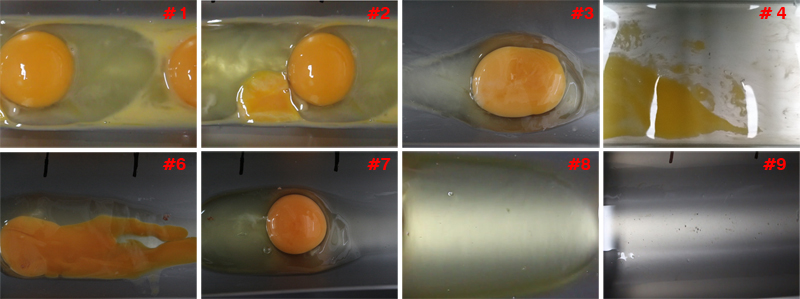
\includegraphics[width=0.8\paperwidth]{8of9}
\caption{Cracked egg product cases.}
\end{figure}

Also, there an additional problem is constituted by chalaza - a usually white element that is attached to egg yolk for in-egg suspension.
Despite the fact, that client decided that chalaza position and amount are irrelevant to him, its appearance may increase difficulty of the recognition problem if identified as parts of damaged egg yolk.

 
\begin{figure}[H]
\centering
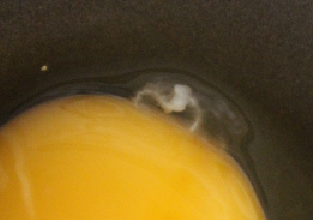
\includegraphics[width=0.4\paperwidth]{chalaza}
\caption{Chalaza attached to egg.}
\end{figure}


\subsection{Techniques of automatic egg quality assessment}

Different techniques for automatic, non-destructive egg quality grading have been investigated.
Among them, the following are worth mentioning:
\begin{itemize}
\item Intelligent systems based on visible-infrared transmittance spectroscopy\cite{agri}
\item Fourier frequency analysis of a vibration-based response on impact force\cite{svm} 
\item Ultrasonic, magnetic resonance, electric resistance, electric nose\cite{nondestr}  
\end{itemize}
All methods listed above require very specific and expensive equipment, are prone to overfitting and take in to account an assumption that does not has to be satisfied for problem considered in this thesis: the egg shell should not be damaged.

Since in this very special case, eggs are already broken, simplified and different methods can be considered.
Initially, two ideas were researched by author of this thesis:
\begin{itemize}
\item Proximity sensor utilization
\item Using laser / narrow light beam 
\end{itemize}
Both methods would identify the intact yolk basing on its height and would not require much processing (an Arduino Uno or other ATMega based circuits might be sufficient).
Nevertheless, both of them had to be rejected, since intact yolks presence in the tested batch is not sufficient for batch accepting – absence of egg yolk parts is also required (see subchapter 2.1).

UWAGA tutaj dwa więcej w tym finally albo trzy; że ta metoda wydaje się być natjańszą najlepsza i polega na umieszczeniu kmaery etc

Finally, using images of the batch obtained from camera and processing it was chosen as a most promising option for further research.



\subsection{Detecting batch state with camera image}

When it comes to assessment of camera image, 4 approaches are widely considered:
\begin{enumerate}
\item Very easy scanning with photo sensors or very low resolution cameras
\item Computer graphics preprocessing and segmentation accompanied with assessment of a parameter (number of pixels, number of feature points, percentage of one region that fills another bigger region and similar)
\item Machine learning approach
\item Neural networks which are used as a special case of either machine learning process or a part of it 
\end{enumerate}
First case was considered, since it could be implemented on Arduino Uno, other ATMega based platform or real-time systems working on PLC controllers such as LOGO! 7, which are often used in factories due to their reliability (apart from Stuxnet-class worms, that has been firstly observed in 2010, no other security threads are believed to exist).
Unfortunately, the problem is more complex than simply deciding whether the product is present or not; or whether the product is yellow or not, thus more advanced processing is required.

Second case will be expanded in the next two chapters and has been chosen as main method that will be implemented and tested in this thesis.

Last two approaches will be tested if the 2nd approach will provide to be insufficient.
It is worth mentioning, that for (3) Support Vector Machines was considered, since it classifies data to exactly two classes (i.e. proper and improper egg mass).

Also, Haar Features Cascade was tested, but data amount obtained for testing was insufficient, and the methods popular implementations are focused on locating the particular object on image rather than on comparing two pattern cases.

(4) Case was considered and the author build a multilayered perceptron network working with MNIST database in order to better understand the method.
The method application will be researched further on beyond the scope of this work.






\section{Batch state detection system design}

\subsection{System structure}
UWAGA zdanie więcej z czego się skłąda (to co jest przy obrazku i refka) i, że kamera zamocowana

A camera will be placed on top of Separator module part, where cracked eggs are transported by sliding to the separating part.


UWAGA tu się coś powieliło
The processing device will use the frames of camera image. Some of the frames will be skipped to reduce amount of data.
Frame-skipping ratio depends on decision algorithm and device performance.

The processing device will use the frames, to make a decision whether or nor the egg batch visible on the frame is acceptable, or represent a badly cracked egg.
A signal will be send to element that will either remove egg batch from the processing plant or let is pass further.
Development of this physical element is done by OVO-TECH company and is not analysed in the thesis. OVO-TECH declared, that having +5V signal for positive batch, and -5V for negative is enough for them to work on their part.


\begin{figure}[H]
\centering
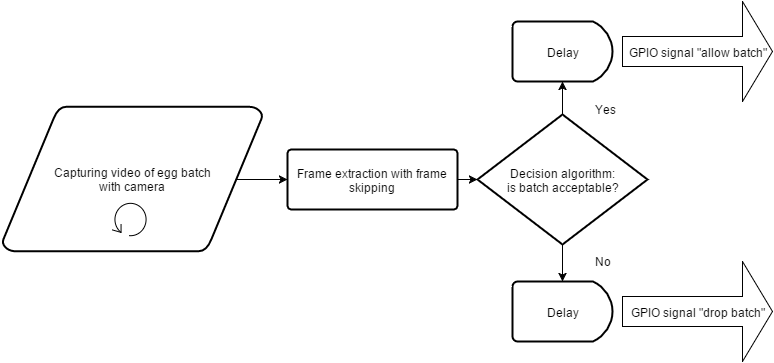
\includegraphics[width=0.8\paperwidth]{system}
\caption{System workflow}
\end{figure}

\begin{figure}[H]
\centering
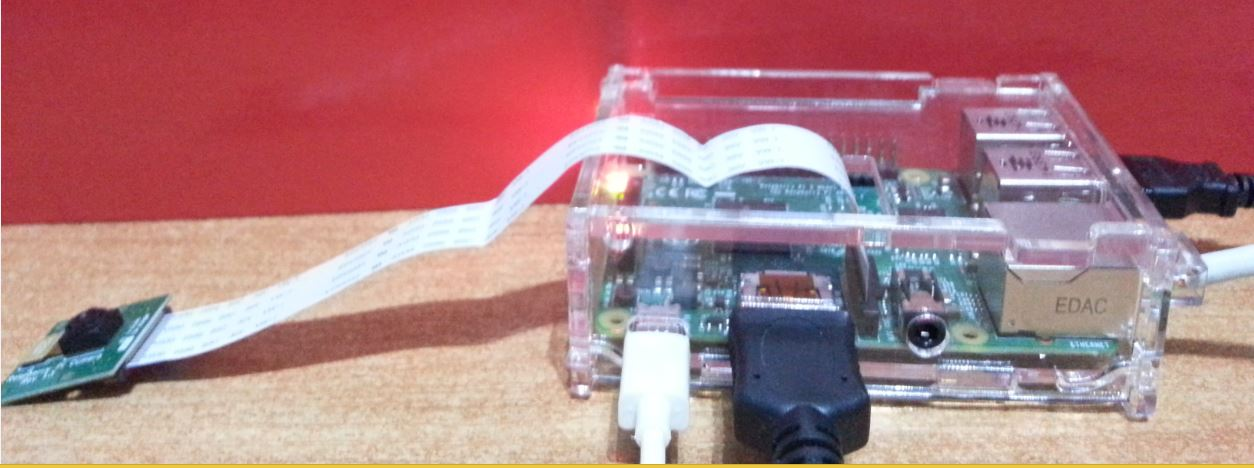
\includegraphics[width=0.8\paperwidth]{phisical}
\caption{Physical system structure - camera and processing device - Raspberry Pi 2 (unmounted from RZ-1 machine)}
\end{figure}


\subsection{Hardware and operating system choice}

Among over 20 available ARM systems, presented below were most interesting as possible to use in the system:
\begin{itemize}
  \item Raspbian - a standard, default Raspberry Pi system in "Jessie" distribution.
  \item Minibian - a Raspbian image that is resource optimised.
  Its current Raspian "Jessie" based version boots in 14secs, use only 29MB RAM and takes 451MB (compared to 1,2GB in original version). GUI, application clients, office suite and other non-necessary packages have been removed. The image is targeted for embedded or server applications (NAS, Web server, electronic applications).
  \item Arch Linux ARM
  \item Gentoo
  \item SliTaz
  \item Windows 10 IoT Core - embedded solution developed by Microsoft. Guarantees extensive technical support.
\end{itemize}

Largest reliability and performance benefits are expected from using realtime-capable systems.
Following solutions are available or developed for Raspberry Pi:

\begin{itemize}
  \item RISC OS
  \item Xenomai
  \item PREEMPT\_RT kernel patch and High Resolution Timers\cite{stackos}
  \item ChibiOS/RT\cite{chibi}
  \item RODOS - an Open Source kernel project developed by the German Aerospace Center and Prof. Montenegro's University\cite{rodos}
\end{itemize}

Nevertheless advanced image processing, GPU access, utilisation of existing graphics libraries might be not available or require amount of effort disproportional to those benefits.
Also, external real-time clock (such as AD9850 Pulse generator) would be required.

The decision was made, to use Raspbian as the operating system, because of its documentation availability and good community support.

Using alternative system operating on Raspberry Pi 2 platform might improve image processing performance. Therefore, more frames per second could be analized, more filters can be applied and higher resolution pictures could be used.
Porting to one of the systems mentioned above will be considered in the future, during the process of designing mass-produced system version.

Following platforms were considered, to be used as processing device and host chosen operating system:

\begin{itemize}
  \item Raspberry Pi 2 - featuring 900 MHz quad-core ARM Cortex-A7 and 1GB RAM, Broadcom VideoCore IV GPU, 4 USB ports, an ethernet port, 40 GPIO ports and camera module socket, its the most available of embedded pc ARM platforms.
  \item Arduino Uno R3 accompanied with DS1307 Real Time Clock - considered, but for now the image processing is to extensive in terms of image processing.
  Having extremely cheap clones (4-20\$ on retail market) that features often stronger ATMega units is an advantage although.
  \item Intel Galileo Gen 2 - based on Intel Quark 32-bit SoC X1000 processor, provides pins-compatible with shields designed for the Arduino Uno R3, what makes communication with other OVO-TECH machine modules easier and allows use of the mentioned above RTC.
  \item PandaBoard - the OMAP4430 features 1 GHz dual-core ARM Cortex-A9 MPCore CPU (a big improvement compared to Cortex-A7 CPU in Raspberry Pi 2), 304 MHz GPU, and 1 GiB DDR2 SDRAM.
  What is interesting, it provides a real-time clock, what makes it a candidate for real-time system (see section 8.1).
  \item BeagleBoard xM - based on dual, 1,5GHz clocked ARM Cortex-A15  + dual ARM M4, 532 MHz GPu, often used with RISC-OS, having cheaper clones with more RAM.It is considered a stronger Raspberry Pi alternative.
  \item Nvidia Jetson TK1 - build on quad ARM Cortex-A15, NVIDIA Kepler 192-cores CUDA GPU, 2 GiB RAM, optimised for OpenGL and OpenCV, equiped with SATA connector.
  TK1 is the strongest available unit, what makes it also the most expensive one.

Raspberry Pi 2 was chosen, due to similar reasons that Raspbian was picked.
Similarly to Raspian, Raspberry Pi 2 may be replaced with different platform inlater design phases, when a prototype is operational and tested.

As for camera module, a standard Raspberry Pi v1.3 5Mpix Camera module was shipped with the board and proves to be more then sufficient in terms of resolution and fps for now.

\end{itemize}




\subsection{Detection algorithm}

Frames are acquired from the camera module.
Two copies of the frame are processed independently. 
UWAGA tutaj jakoś zaznacz, że każda z kopii jest jest osobno wypunktowana

\begin{description}
  \item[Firstly,]one channel is extracted from the image.
  Its state is passed further as image, along all the steps.
  \item[Secondly,]the channel is a subject to preprocessing, that eliminates the unimportant data and reduces the data dimensionality. 
  Amount of noise is reduced.
  \item[Thirdly,]the image is segmentation, and the shape recognition methods are used to detect existence, position and size of the egg yolk.
  \item[Independently,]other copy of the image is a subject to different color scale.
  \item[Then,]only one channel is extracted from the image
  \item[Finally,]the information from first copy is used to remove intact egg region from second copy.The first copy is no longer needed and its resources are freed.
\end{description}

Chosen channel of transformed second copy (with intact egg excluded) serve as the only image now.
It is processed in a following way:

\begin{description}
  \item[Firstly,]an attempt is made to filter out the light reflections and flares from the image.
  Hopefully, during the further development, above artefacts can be removed in a physical way, by mounting and lighting the device in a very specific way.
  For now nevertheless, this step is necessary.
  \item[Secondly,]image is segmentated with thresholding.
  \item[Thirdly,]noise (defined as small blobs) is deleted.
  \item[Finally,]the obtained image is expected to contain only unwanted, damaged egg mass.
  Amount of pixels containing it is counted.
  \item[Decision] is made basing on the obtained amount.
  It takes a form of signal sent to physical element that either removes the egg batch or let it through.
\end{description}

The best obtained combination of preprocessing, segmentation and grading parameters will be used in a final algorithm that will be implemented in Raspberry Pi 2 device with camera module, and than tested in the Rz-1 processing plant.


\begin{figure}[H]
\centering
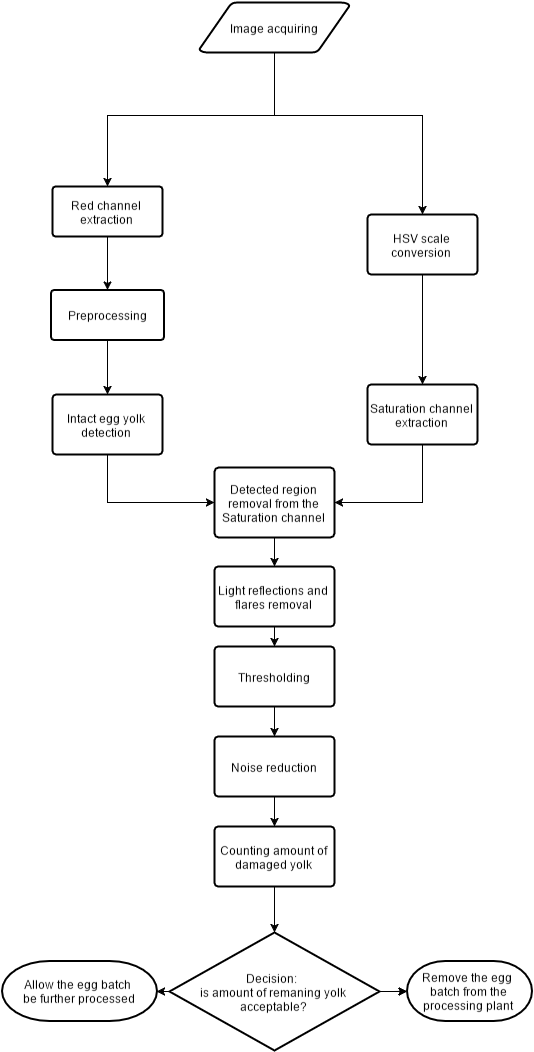
\includegraphics[width=0.5\paperwidth]{algorithmV}
\caption{Detection Algorithm}
\end{figure}


\subsection{Software choice}
Decision have been made, to utilise OpenCV computer vision library for batch state recognition.
OepnCV is designed for computational efficiency, with strong focus on real-time applications.
It has been written in optimised C and takes advantages of multicore processors.
It provides simple-to-use interface that enables building sophisticated computer vision solutions.
The library features more than 500 functions that process images, a general Machine Learning Library (including Multilayered Perceptron Networks).
It is used since 1999 by major institutions such as Stanford University and is maintained and developed by specialists from companies such us IBM, Microsoft, Intel, Sony, Siemens, and Google.\cite{learnopencv}

First recognition attempts were done by the author of thesis using Android 4.3 running on Samsung N7100 Galaxy Note II smartphone, utilising its build in camera.
The initial code was written with use of Java distribution of OpenCV library, as well as Android SDK.
Sadly, the performance of developed pre-prototype was very poor and a single frame was processed in more than 3 seconds.
Another version was build in a way that most resource consuming operations (such us Hough Circle Transform and all array operations) were rewritten in C language.
For that purpose original C version of OpenCV was utilised, as well as NDK (Native Development Kit for Android).

Nevertheless, author of this thesis, decided that despite Android availability for embedded platforms, it is no a platform suitable for factory tasks, due to big overhead, long booting and variety of functions that will not be utilised.

Raspbian Linux "Jessie" distribution was picked as the adequate one to host recognition algorithm accompanied with Python 2.7 language.
Python is well supported on Raspian, it produces small amount of code, and can be executed fast in terms of computational time if the specific C-written functions are called.\cite{performance}
For author, a case occurred, that 39-lines code snippet that recognise nested regions of image, written in C took only 6 code lines after rewriting it in Python.


\section{Egg yolk detection}
\subsection{General idea}
An egg yolk, when intact and fresh can be approximated with sphere which projects as circle-like shape on 2D image.
Methods presented below enable to filter out the unnecessary noise, simplify the image and detect the yolk shape.
While not all of them were used in the final detection algorithm, they were giving promising results on the early stage prototypes.

Parameters, which values have to be found to correctly apply the methods are indicated with \textbf{bold font}.

Following methods treat images as 1, 8, or 24-bit encoded matrices, thus both terms are used synonymously.
x and y denote pixel position.
\subsection{Extracting channels}
In digital graphics color information is usually stored as a value from RGB (or BGR) additive color space.
It means, that three numbers represent amount of red, green, anb blue subcolors that combined constitute a visible color.
For this algorithm sake, it is assumed that every one of this numbers takes values from 0-255 interval and is encoded by 8bits, what sums to 24bit encoding for every RGB pixel.

Alternatively, a simplified information may be processed: a grayscale image is made of pixels encoded by a single number that denotes the colors distance from being completely black; the higher is the number, the closer to being white it is.
8bit encryption has been chosen for grayscale images.

There is also an option to store binary black-and-white image with 1bit encoding (0 picked for black, 1 for white).
 
A channel in this context is a grayscale image that represents intensity of single subcolor in RGB space. 
For example, a red channel is an image, in which 255 constitutes red pixel, and 0 means that pixel has no red subcolor.

It is suspected by the author that using a single channel instead of commonly used RGB image may is more efficient and some unnecessary information in dropped.
Particularity, an egg yolk that is visually yellow or red my be favoured in red or green channel.

\begin{figure}[H]
\centering
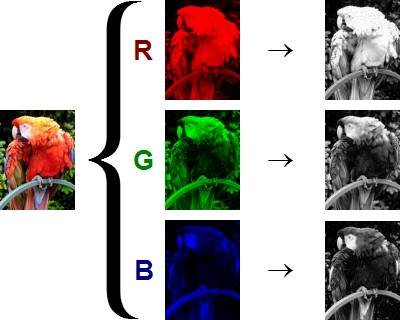
\includegraphics[width=0.4\paperwidth]{rgb}
\caption{Three channels of RGB image. Src: www.commons.wikimedia.org}
\end{figure}


\subsection{HSV scale conversion}

Extending assumption from previous subchapter led author to belive that using a color space different than RGB might be more effective in recognition process.
It might occur, that the problem of assigning color values associated with egg yolk is either linearly separable or close to being such, and thus extracting only those pixels that constitute egg yolk might be possible.

HSV cylindrical color space is known as being exceptionally suitable as a preprocessing method used before image segmentation \cite{hsv}

In HSV color is represented by Hue (angle of a point on a cylinder), Saturation (a radius of a point) and Value (height of the point).

Hue is defined as "the degree to which a stimulus can be described as similar to or different from stimuli that are described as red, green, blue, and yellow"\cite{hue}.
Saturation stands for intensity of a particular hue.
Value is also defined as darkness of the color and is often treated as reverse grayscale channel.


\begin{figure}[H]
\centering
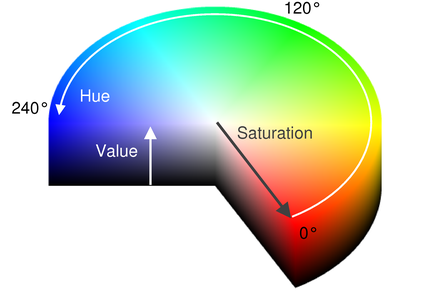
\includegraphics[width=0.4\paperwidth]{hsv}
\caption{HSV Cylinder. Src: www.doc.qt.io}
\end{figure}


\subsection{Circle Hough Transform (CHT)}
Circle Hough Transform is an algorithm used for retrieving 3 parameters defining a circle-like shape on images\cite{hgtcv} : 
- (xc, yc) - position of shapes center
- r - its radius

To understand the way CHT works, simplified case is considered:
The image is 1-bit encoded; the radius r and position (xp,yp) of a point lying on the searched circle are known.
Potential circles space is created by treating points on a circle of radius r centered in (xp,yp) as centers for potential circles.
For every potential circle, number of intersecting points is counted.
The potential circle with largest number of intersections is chosen as the best fitting one.

 
\begin{figure}[H]
\centering
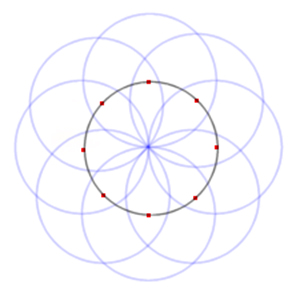
\includegraphics[width=0.4\paperwidth]{space}
\caption{Potential circles space\cite{craters}}
\end{figure}

In the full cases, such procedure is repeated for every image point, and the intersections numbers are stored in accumulation matrix.\cite{hgt}
To reduce computation time and false detection rate, minimum distance between image centers is given as a parameter \textbf{minDist}.
Threshold value \textbf{param2} is defined as minimum number of intersections to treat circle candidate as detected circle.
 
\begin{figure}[H]
\centering
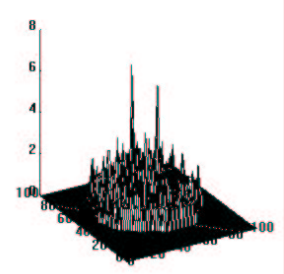
\includegraphics[width=0.4\paperwidth]{accu}
\caption{Accumulation matrix with two good circle candidates\cite{hgt}}
\end{figure}

If r is unknown, min-radius and max-radius parameters are defined, and the algorithm repeats the procedure for all possible integer r in range of above parameters.
OpenCV utilizes Canny edge detector for finding the potential intersection points, thus operates not only on 1-bit images, but also in 8-bit grayscale and 24-bit bgr images and provides smaller number of false positives.\cite{mastercv}
\textbf{param1} is introduced as higher threshold for Canny edge detector, while the lower threshold is set to 0.5 * param-1\cite{fd} .


\subsection{Erosion and Dilatation}
Erosion and dilatation are two morphological filters that enable to filter out unnecessary noise from the image.
Combined, they leave the core information (biggest blobs) intact or amplified, while small elements are deleted.
It is easily applied to binary images:
A ROI (region of interest, a rectangular part of image) moves through image pixel by pixel and is compared to previously defined kernel (binary matrix, usually symmetric with respect to both diagonals).

 
\begin{figure}[H]
\centering
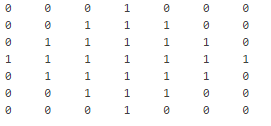
\includegraphics[width=0.4\paperwidth]{diam}
\caption{A diamond-shaped kernel\cite{morph}}
\end{figure}

The consecutive pixels of on ROI that matches kernel elements with value 0 remain intact.
Pixels of ROI that matches kernel 1-valued elements changes to:
1-ns if at least one of them is 1 for Dilatation
0-s if at least one of them is 0 for Erosion.

Erosion gives the effect of ‘shrinking’ the objects (and if they are small enough, they are deleted).
Dilatation makes the objects bigger.

 
\begin{figure}[H]
\centering

\includegraphics[width=0.4\paperwidth]{lett}
\caption{Original image, eroded image, dilated image.\cite{erdil}}
\end{figure}


When these methods are used multiple times, and convoluted, they filter out the noise.
Using erosion and dilatation with the same kernel one ofter another is called opening.
Perimeter Determination and Skeletonization are widely used contour detection functions which utilize erosion and dilatation\cite{erdil}.


\subsection{Gaussian blur}

Gaussian blur is obtained by convoluting pixel with gauss function values. 

It reduces noise, detail and filters out the high frequencies what makes it a low pass filter.\cite{cv}

Gaussian blur drastically reduces number of false-positive Hough circles detections. It nevertheless should be coupled with sharpening to reduce false-negative cases.\cite{cnoisy} 


\begin{figure}[H]
\centering
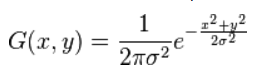
\includegraphics[width=0.4\paperwidth]{gauss}
\caption{Gauss function in two dimension\cite{featproc}}
\end{figure}


sigma, ksize.width, ksize.height  parameters are introduced.
Ksize stands for size of precomputed kernel, that is convoluted with ROIs on the image.

The term ‘convolution’ might be misleading and for the scope of image processing tasks is defined as piecewise multiplying two matrices and than summing the obtained values:

 
\begin{figure}[H]
\centering
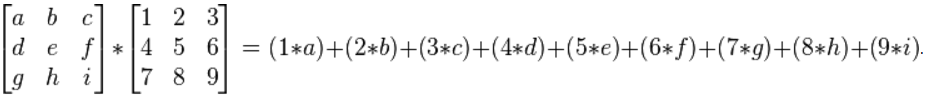
\includegraphics[width=0.8\paperwidth]{conv}
\caption{Convolution of 3x3 matrices\cite{gimp}}
\end{figure}

 
\begin{figure}[H]
\centering
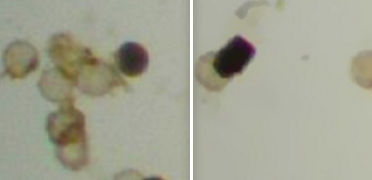
\includegraphics[width=0.4\paperwidth]{micro}
\caption{Microscope image before and after applying gaussian filter\cite{cnoisy}}
\end{figure}

  



\subsection{Methods execution}
\lstinputlisting[language=Python]{yolk.py}
UWAGA więcej komentarza w methods execution

\begin{figure}[H]
\centering
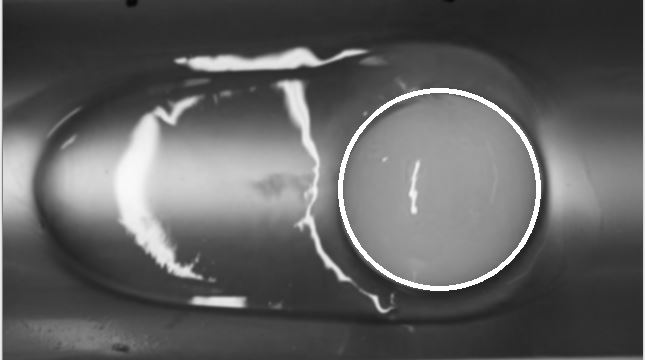
\includegraphics[width=0.4\paperwidth]{detected}
\caption{Properly detected intact egg yolk\cite{cnoisy}}
\end{figure}


\section{Contaminated product recognition}
Methods described in previous chapter are used for contaminated product recognition, as well as two more presented below:

\subsection{Subtracting yolk image}
Subtracting image of detected intact egg yolks from the general image outputs an image that holds only unwanted egg yolk, egg white and its surrounding.
Therefore, the problem would be reduced to simple assessing the amount of remaining egg yolk and comparing it to a threshold value for acceptable bad yolk amount.

The initial implementation for this methods was supposed to be obtained by filling the image with empty circles detected in the previous chapter.
Unfortunately, it has been sentimentally tested, that egg yolk is reflecting some yellow light on it's surroundings and it is very hard to filter them out, thus a bigger area is subtracted.
Instead of circles, empty rectangles are drawn on the analysed image. The rectangles fill the whole image height (since eggs do not slide parallely due to transportation slope design), and their width is equal to detected yolks diameter summed with an offset that covers reflecting light. The rectangles centeres are equal to yolk centers.

\subsection{Thresholding}

Thresholding is a simple case of image segmentation.
It can be used to convert one channel (in most cases grayscale) image to binary image.
The basic binary thresholding mode sets every pixel of destination matrix to:
\begin{itemize}
\item 0 if the source matrix value is smaller than threshold (integer parameter)
\item 1 if the source matrix value is bigger than threshold.
\end{itemize}
The truncate version sets every pixel of destination matrix to
\begin{itemize}
\item threshold if the source matrix value is smaller than threshold, or
\item leaves it unaltered otherwise.
\end{itemize}
Various modes and modifications are used depending on coding schema and colors distribution.
  
\begin{figure}[H]
\centering
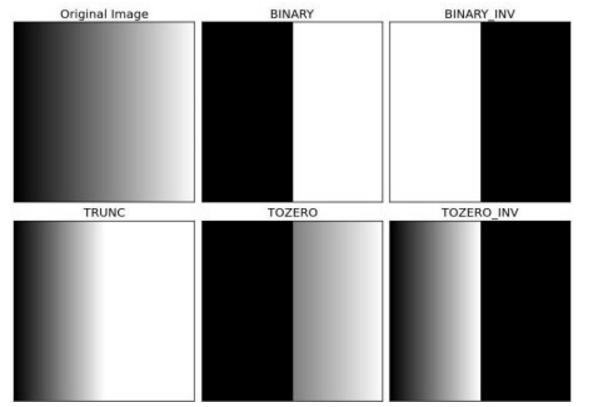
\includegraphics[width=0.4\paperwidth]{thr}
\caption{Different Thresholding modes generated with Metaplotlib}
\end{figure}

UWAGA obrazki mają być bardziej zwarte w thresholdingu

Finding optimal threshold value finding is a time consuming process and it often gives satisfactory results only for small set of images.
Therefore Otsu Binarization algorithm for automatically selecting threshold is used.

Moreover using one threshold value for whole image may not work properly if the lighting conditions differ in different image areas.\cite{thre}
Adaptive Thresholding utilize different threshold values for different ROIs.
Two modes are often used: Adaptive Mean and Adaptive Gaussian.
First compute threshold value as mean of neighbourhood values.
Second uses weighted sum neighbourhood values.
 
\begin{figure}[H]
\centering
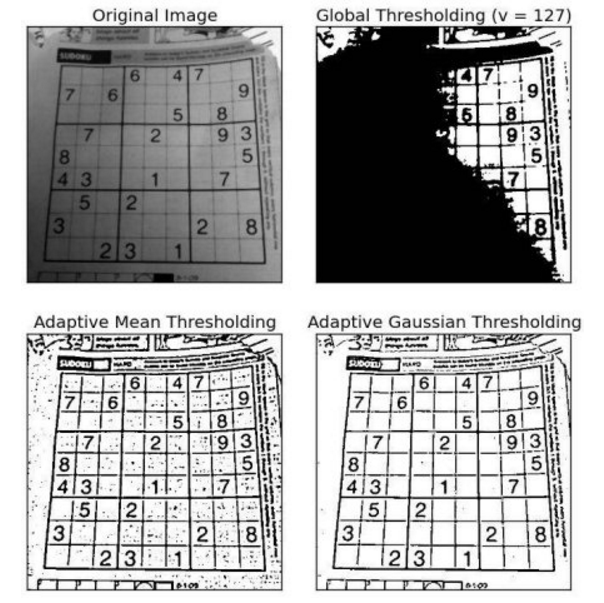
\includegraphics[width=0.4\paperwidth]{thremeth}
\caption{Threshold computing methods12\cite{thre}}
\end{figure}
 
\begin{figure}[H]
\centering
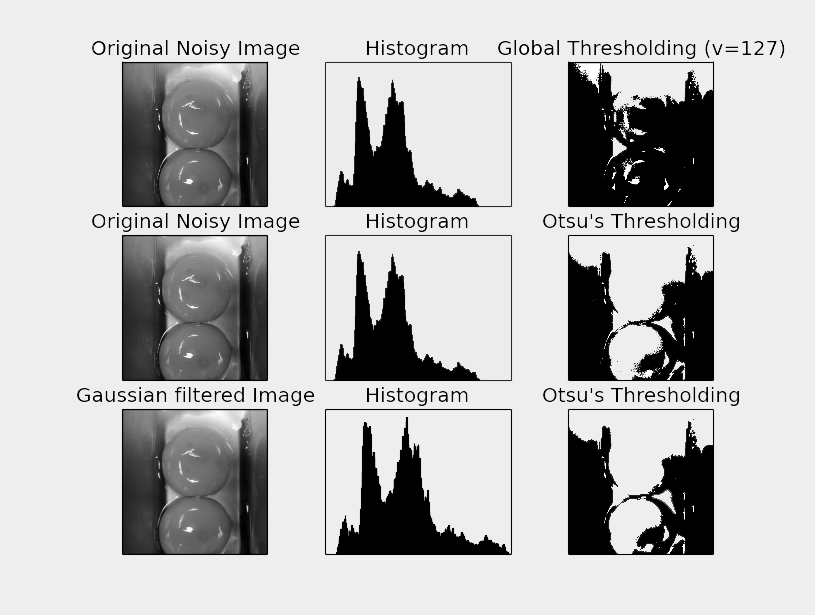
\includegraphics[width=0.4\paperwidth]{diffthr}
\caption{Different thresholding applied
Fig. generated with Metaplotlib}
\end{figure}

\begin{figure}[H]
\centering
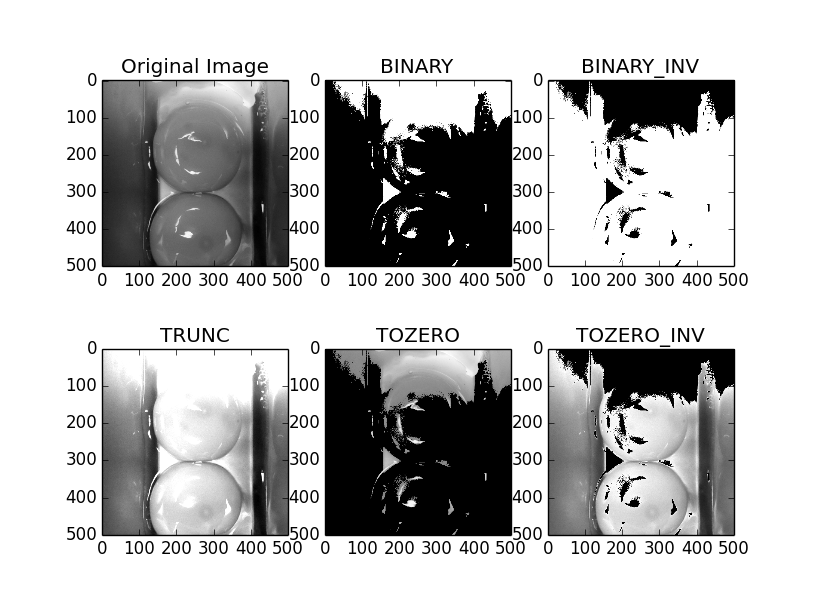
\includegraphics[width=0.4\paperwidth]{gray}
\caption{Inefficient thresholding of grayscale image}
\end{figure}

\begin{figure}[H]
\centering
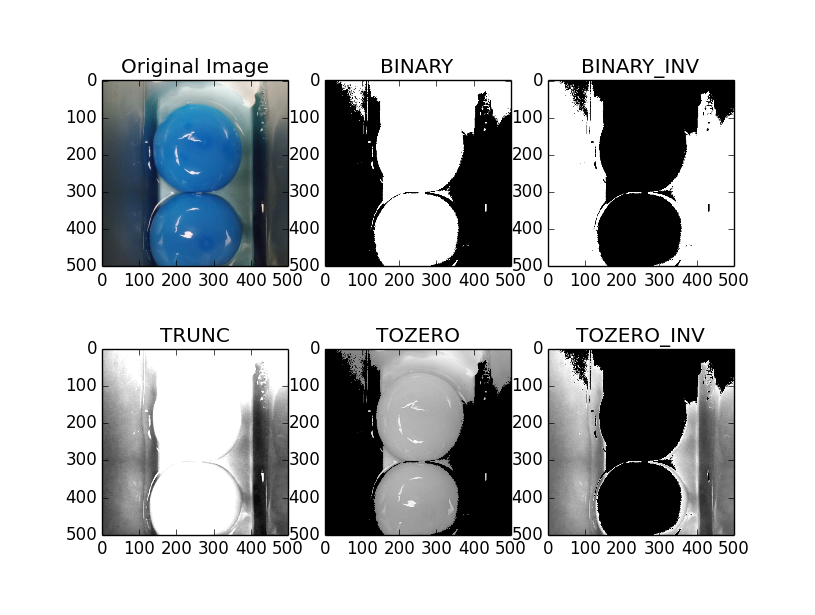
\includegraphics[width=0.4\paperwidth]{red}
\caption{Much more effective thresholding of red channel image}
\end{figure}

For more general cases (i.e. multichannel images, assigning more colors) clustering method known as k-means is widely used.\cite{lesscv}
 
\begin{figure}[H]
\centering
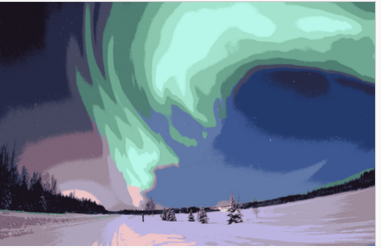
\includegraphics[width=0.4\paperwidth]{kmeans}
\caption{K-means clustering method for k = 16\cite{segm}}
\end{figure}
\subsection{Methods execution}
UWAGA dużo więcej komentarza w methods execution
\lstinputlisting[language=Python]{contaminated.py}

\begin{figure}[H]
\centering

\includegraphics[width=0.4\paperwidth]{bad}
\caption{Properly segmented damaged yolk mass}
\end{figure}

\section{Choosing detection system parameters}
\subsection{Manual parameters optimisation}

There exist a set of parameters that define the mode, that previously explained methods operate as well as their insensitivity.
Finding optimal values of this parameters is a hard task, since for example CHT method was not able to found a single egg yolk with default numbers.


Few similar scripts were developed, that displayed over 500 sample pictures pictures (provided by OVO-TECH) for 0.3 second each in a loop.
Various trackbars was displayed above the frames, with every trackbar corresponding to one parameter that is supposed to be chosen.
Beside, the already transformed frames after transformations were shown.
The expert was reviewing the output while changing the trackbar positions to obtain an image that segmentates the egg yolk properly.

\begin{figure}[H]
\centering
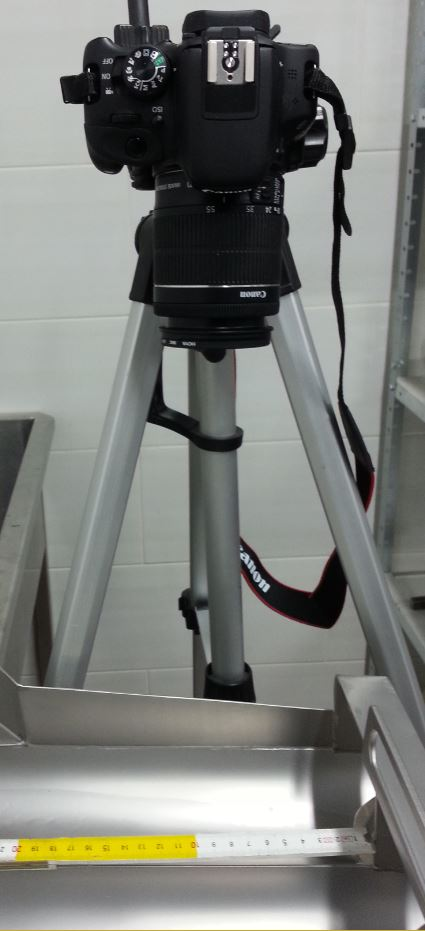
\includegraphics[width=0.2\paperwidth]{samples}
\caption{Obtaining a set of sample pictures. Another set was obtained using Raspberry Pi camera.}
\end{figure}

\begin{figure}[H]
\centering
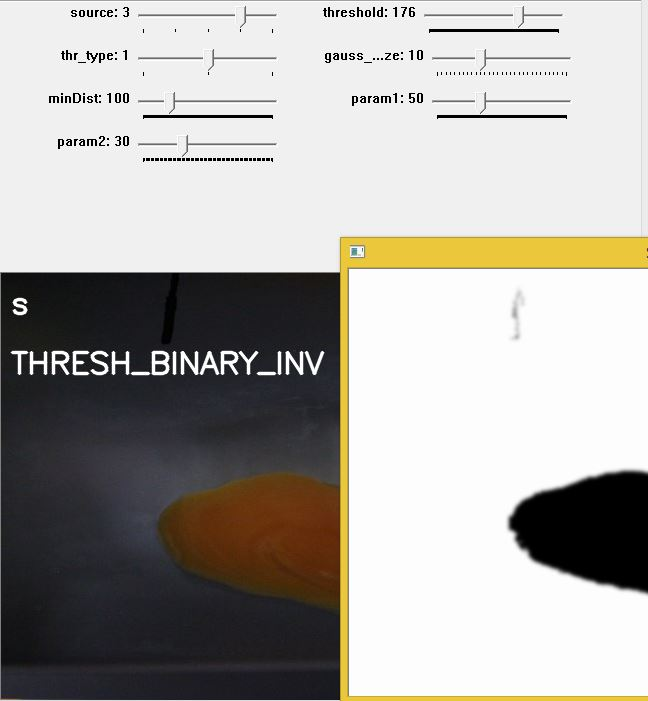
\includegraphics[width=0.5\paperwidth]{manual}
\caption{One of the scripts used for manual parameter interval finding}
\end{figure}

Script crucial fragments:
UWAGA wywalić trackbary a napisać, że eksprt zmienial wartosci parametrow
\lstinputlisting[language=Python]{trackbars.py}

Unfortunately, while some parameters sets worked fine for some image sets, they failed with another ones.
Nevertheless, the interesting intervals were obtained for each trackbar. These intervals guaranteed that at least some of the graded images are segmentated in expected way.
This method resulted in excluding most parameters values and vastly reducing the optimising problem size.

\subsection{Automatic parameters optimisation}

A decision was made, to automatise process of assessing the segmentation and detection efficiency to get to optimal set of parameters.
This process was done twice:
\begin{description}
\item[Firstly,] the egg yolk detection process was optimised.
\item[Secondly,] the contaminated product detection utilising the previously optimised egg yolk detector was perfected.
\end{description}

To accomplish first objective, available images were divided into 3 subsets for first process:
\begin{itemize}
\item 0 intact yolks visible in a frame
\item 1 egg present
\item 2 eggs present
\end{itemize}
For the whole set, the recognition error was defined  as sum of missdetections for every subset.
A similar procedure was conducted for second objective: the same images were divided into following subsets:
\begin{itemize}
\item Contaminated batches
\item Batches with either only intact eggs or no egg mass at all
\end{itemize}
Error was defined as false negatives (good batch recognised as bad batch) number summed with false positives number multiplied by 3.
Multiplication by '3' weight was conducted on false positives, since keeping the product clean is more important for the client, that utilising all the egg mass. 

A script was developed, that automatically loaded the images and graded them for different parameter values.
This process was very expensive in terms of processing time, and the parameters range and step was chosen to fill a night of i7-3520M 8GB RAM computer work.
It was computed in a following way: elapsed time of one full imageset testing multiplied by number of possible parameter sets.
The process was repeated by the author multiple times with different parameter intervals discovered in a process descried in previous subsection.
Various effort were made by the author to optimise imageset grading process, so bigger variety of parameters can be checked.
Initially, files were open prior to every image evaluation, later on all the images were loaded once, and every processing (channel splinting, colorscale conversion) was conducted before execution of the code nested in multiple loops.

Crucial parts of the testing code:
\lstinputlisting[language=Python]{script.py}


\subsection{Overfitting}
Overfitting is an unwanted effect that appears often in statistics and supervised machine learning.
Overfitting means, that parameters of some model are fitting the specific modelled data case, rather than the general model.

In this case it means, that the parameters of image processing that were found, maximise the recognition efficiency for the data provided by OVO-TECH, while a new data (with different kind of eggs, different kind of noise or with images made in different conditions) can be classified in improper way.

Overfitting occurs mostly if:
\begin{itemize}
\item A set of sample data is too small
\item A set of sample data is not diverse enough
\item No regularisation or cross-validation methods are used
\end{itemize}

To reduce this effect, author used different dataset for getting the transform parameters, and different set (excluded 10\% of data from every sample subset) for assessing the recognition quality.

During prototype in factory testing and further development this issue will be addressed in extended way.
\subsection{Results}
The following parameter values were obtained in a process of automatic parameters optimisation executed for on 195 sample photos that depict properly cracked egg and 388 depicting bad batches.
The recognition accuracy maximised during optimisation process was 91,25\%, and the recognition accuracy on the testing set of 57 images was 84,2%.
\begin{figure}[H]
\centering
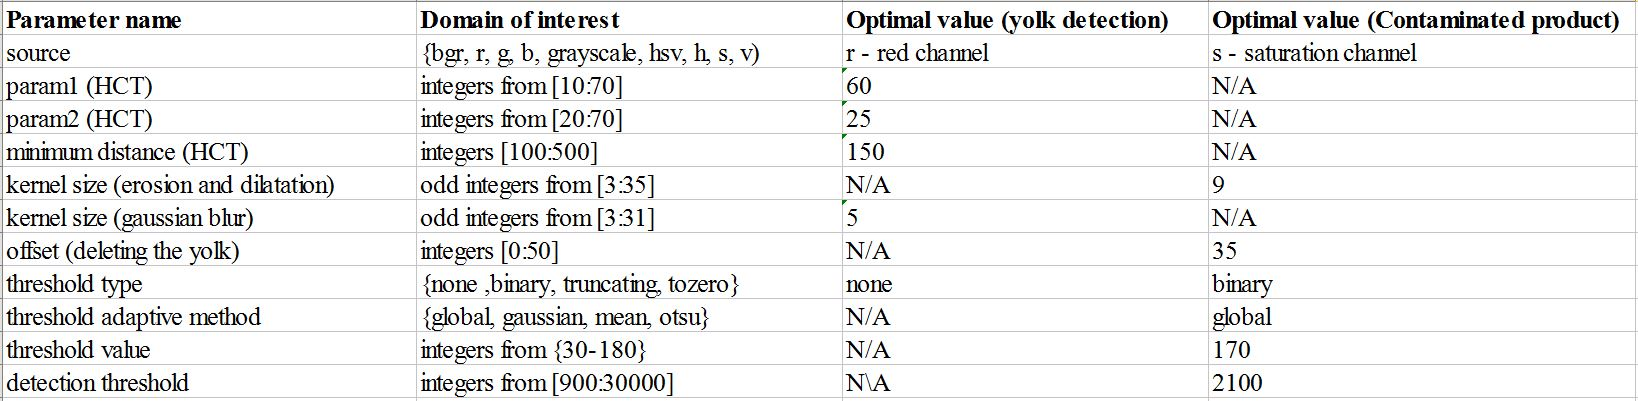
\includegraphics[width=0.8\paperwidth]{params}
\caption{Parameter values obtained in automatic parameters optimisation}
\end{figure}



\section{System implementation}
\subsection{Hardware and OS issues}

Initially, hardware platform was connected to LG 27MP35 display through HDMI, iBox keyboard and mouse via USB. 
MicroSD SanDisk 8GB card (with EMTEC MicroSD Adapter)was used as a hard drive for operating system. 
TP Link WN725N USB WiFi adapter was used.

Device was powered from laptop USB port via microUSB cord, that has to be shaped to fit into Raspberry Pi casing.



\begin{figure}[H]
\centering
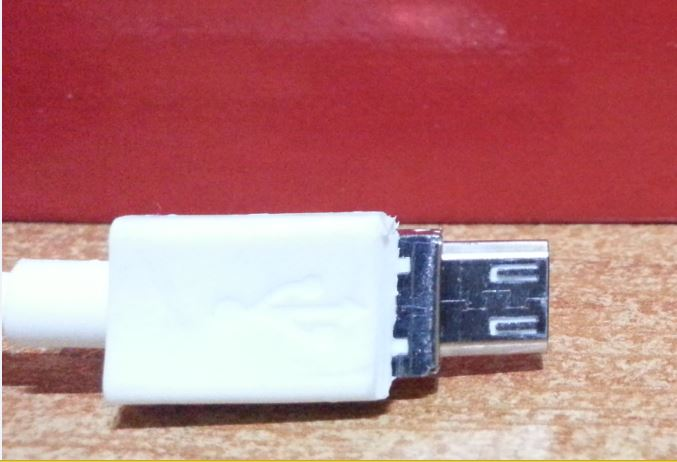
\includegraphics[width=0.3\paperwidth]{cable}
\caption{Cord had to be shaped with a knife to fit into Raspberry Pi casing}
\end{figure}

Raspberry Pi Camera Rev 1.3 was picked to be used as a camera module. 

\begin{figure}[H]
\centering
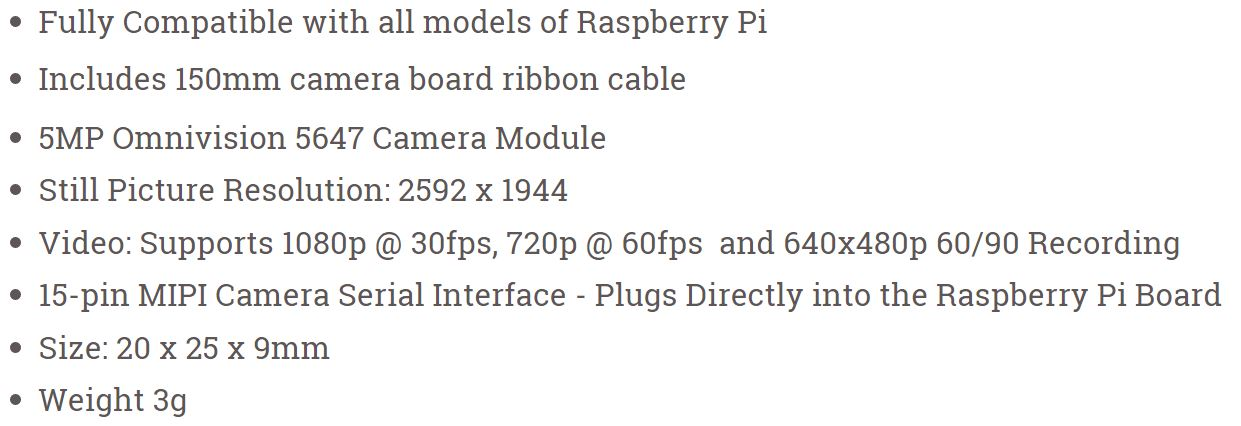
\includegraphics[width=0.5\paperwidth]{features}
\caption{Camera module features. Src: www.modmypi.com}
\end{figure}

To install Raspian system on the chosen platform, SD card had to be prepared.
Diskpart windows tool has been used to delete all partitions and create a new one on SD card, since regular format was not enough to clear old Raspian installation - only 700 MB out of 8GB could be reclaimed that way.
The card partition was formatted in fat32 file system.
Later on, OS installer automatically partition it to both fat32 and ext4 filesystems partitions.
Clean "Jessie" - "NOOBS" distribution in .zip archive was copied to drive.

Next, OS setup was conducted on device.
Standard updates were conducted after WiFi network setup:
\begin{lstlisting}
$ sudo apt-get update
$ sudo apt-get upgrade
$ sudo rpi-update
\end{lstlisting}

Unfortunately, the screen was either blinking or had unreadable 320x240 resolution on 27MP35 display, and on tested L227WT display and EB-1761W projector displayed either ‘out of range’ error, or no image at all.
Commenting the 
\begin{lstlisting}
hdmi_mode=16
hdmi_group=1 
\end{lstlisting}
lines in boot/config.txt file and rebooting enabled devices to work properly in VGA mode.

Later on, the device was accessed via Putty SSH using either router with DHPC enabled or direct Ethernet to PC computer using static 169.254.1.1 ip reserved for direct devices connecting.

Xming software with lxsession was using for x11 forwarding - displaying the OS and GUIs on larger PC, so the egg flow could be viewed.

\subsection{Python and OpenCV configuration}

Downloading and building OpenCV with all its dependencies was along process (operations elapsing over 8h, not including the authors involvement).
Following commands were executed:

\begin{lstlisting}
$ sudo apt-get install build-essential cmake pkg-config
$ sudo apt-get install libjpeg8-dev libtiff4-dev libjasper-dev libpng12-dev
$ sudo apt-get install libgtk2.0-dev
$ sudo apt-get install libavcodec-dev libavformat-dev libswscale-dev libv4l-dev
$ sudo apt-get install libatlas-base-dev gfortran
$ wget https://bootstrap.pypa.io/get-pip.py
$ sudo python get-pip.py
$ sudo pip install virtualenv virtualenvwrapper
$ sudo rm -rf ~/.cache/pip
\end{lstlisting}
Following lines were added to ~/.profile file:
\begin{lstlisting}
# virtualenv and virtualenvwrapper
export WORKON_HOME=$HOME/.virtualenvs
source /usr/local/bin/virtualenvwrapper.sh
\end{lstlisting}
Than, following commands were executed:
\begin{lstlisting}
$ source ~/.profile
$ mkvirtualenv cv
$ sudo apt-get install python2.7-dev
$ pip install numpy
$ wget -O opencv-2.4.10.zip http://sourceforge.net/projects/opencvlibrary/files/opencv-unix/2.4.10/opencv-2.4.10.zip/download
$ unzip opencv-2.4.10.zip
$ cd opencv-2.4.10
$ mkdir build
$ cd build
$ cmake -D CMAKE_BUILD_TYPE=RELEASE -D CMAKE_INSTALL_PREFIX=/usr/local -D BUILD_NEW_PYTHON_SUPPORT=ON -D INSTALL_C_EXAMPLES=ON -D INSTALL_PYTHON_EXAMPLES=ON  -D BUILD_EXAMPLES=ON ..
$ make
$ sudo make install
$ sudo ldconfig
$ cd ~/.virtualenvs/cv/lib/python2.7/site-packages/
$ ln -s /usr/local/lib/python2.7/site-packages/cv2.so cv2.so
$ ln -s /usr/local/lib/python2.7/site-packages/cv.py cv.py
$ workon cv
$ python
\end{lstlisting}

\subsection{Code deployment}

UWAGA nie deployment tylko implementation i więcej trochę

\lstinputlisting[language=Python]{rpi.py}
\section{Further research and development}

Work on the solution developed in this thesis will be continued further on by the author and OVO-TECH company.
The following alternative approaches and improvements in detection system will be taken into consideration

\subsection{Server and logging}
Gathering the data about egg quality, recognition performance and effectiveness is a possibility that has to be addressed.
Raspberry Pi 2 platform is capable of working as a server and thus provide system manufacturer a remote access to the its operations.

Such process may generate additional benefit, which is deciding whether or not the processed eggs quality is good.

Ovo-tech reported cases of unreliable egg suppliers, that shipped old, misclassified eggs either purposefully or unwillingly to the bakery companies.
Such situation would be detected by monitoring statistics of how big percentage of processed eggs are badly broken.
\subsection{One month prototype testing and environment of work tuning}

The prototype will be attached to the rz-1 machine operating at OVO-TECH headquarters for a month.
During that time, led lights will indicate proper and improper egg batch.
Recognition efficiency is now > 80\%. Two cases may occur, when the device is operating in working environment:
\begin{enumerate}
\item Recognising efficiency will rise dramatically, since the camera position will be fixed, and the background (separation module slope) will have uniform facture and color.
The data provided by OVO-TECH for prototype construction covered various situations and backgrounds that will be invariant in factory application.
\item Recognising efficiency will drop, due to varying egg quality, color and shape (the overfitting problem).
\end{enumerate}

Two things will be done to improve image material quality registered by camera:
\begin{itemize}
\item Polarizing filter will be attached to the camera.
It should eliminate or drastically decrease amount of white light reflexes.
Those reflexes that make yolk appear as non-yolk at segmentated image.
\item Lighting will be uniform due to covering camera and a fragment of transportation slope in a box-like container with invariant, non-shadowing lights inside of it.
\end{itemize}

Author and Ovo-tech expect a large efficiency increase after those modifications.
\subsection{Testing new approaches}

Two approaches have came up after the prototype development and are to be implemented and tested:

\begin{itemize}
\item Circularity testing - height of the segmented yolk flow can be treated as a circle diameter. Than, area of obtained circle can be compared to area of observed egg yolk. If the difference is significant, it indicates that observed blob is not a whole egg.
Using a derived method for positioning the center of such circle might work better than methods used up to now if a noncomplete part of egg is visible at the image.
\item Watershed algorithm accompanied with extracting peaks of Euclidean Distance Transform is believed to work better than contour detection and thresholding methods with touching or overlapping objects.
It might provide efficiency boost in case of RZ-1 processing plant operating in modes faster than precise mode.\cite{watershed}
\end{itemize}

\subsection{Obtaining more image data and parameters tuning}

Larger dataset of more different egg types will enable to better tune the processing parameters.
Since there are more than 10 parameters to adjust and the number of operations that are required rise exponentially with parameters number and is multiplied by sample amount, optimising such multivariate function is a hard task.
Genetic algorithms are known to be a good metaheuristics for such tasks and should give better results in much less computation time that brute force parameter testing.
Author developed a program that implements genetic algorithm in Java, that optimises 1,2 and 3-variate functions to understand and learn the genetic algorithm concepts.
Further on, a ready, popular library will be used for this purpose: a DEAP genetic programming library for Python.


\begin{figure}[H]
\centering
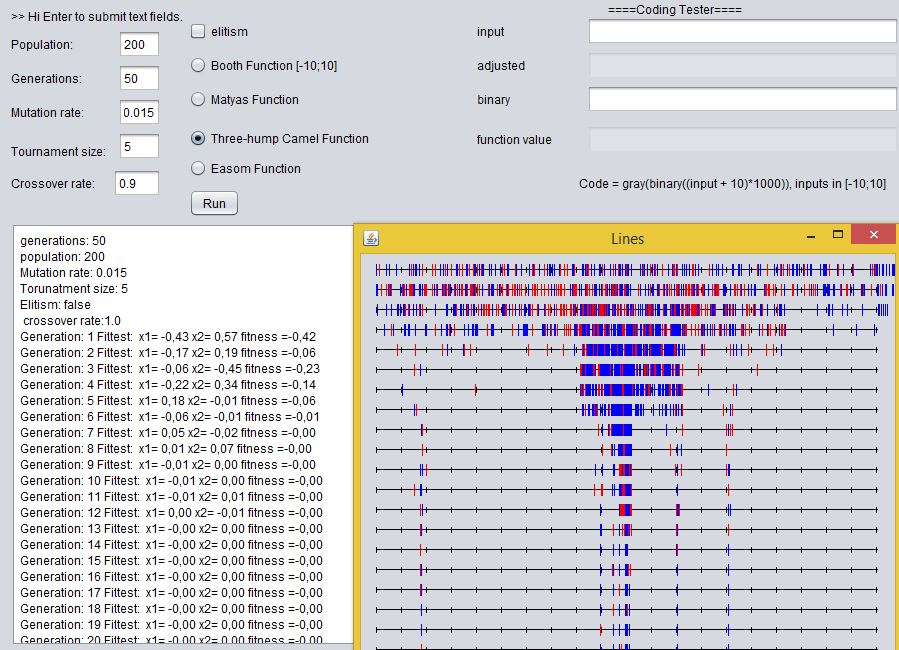
\includegraphics[width=0.7\paperwidth]{genetic}
\caption{Screen of Java genetic function optimiser written by author of this thesis \cite{morph}}
\end{figure}


\subsection{Machine learning}

\section{Conclusions}

Following results were obtained in the system designing, tuning and testing process:
\begin{enumerate}
\item Recognising egg-batch state using camera image is an adequate method of solving the problem of imperfect egg-white separation.
\item Simple image processing methods are cable of obtaining image recognition efficiency higher than 84\% on this problem, even if lighting and camera placement conditions are unfavourable.
\item An operational prototype device was constructed and implemented. It will be tested and improved further in order to introduce it to mass production. OVO-TECH will be expanding its R\&D section to obtain that goal.
\end{enumerate}

Both the project goals has been achieved.


All the Web. sources have been checked for availability in November 2015.
Web links are not included if articles are to be immediately found with search engines, which is consistent to MLN referencing convention.
For modified web documents, date of last modification is shown.
UWAGA dopisz ze zdjecia own materialow sa nieopisane

\begin{thebibliography}{9}


\bibitem{trillion}
Ghose T.
\textit{Could Science Hatch the Perfect Fake Egg?}  LiveScience Web. 2013
 
\bibitem{eggprop} 
Berry D.
\textit{Egg product functional properties} 
American Egg Board Web. 2013

\bibitem{agri} 
Mehdizadeha S., Minaeib S., Hancockc N. H. ,Torshizid M.
\textit{Information Processing in Agriculture}, Volume 1, Issue 2 
Print. 2014

\bibitem{svm} 
Deng X., Wang Q., Chen H., Xie H.
\textit{Eggshell crack detection using a wavelet-based support vector machine} Comput Electron Agric, Print. 2010

\bibitem{nondestr} 
Ketelaerea B.,Bamelisa F., Kempsa1 B., Decuyperea1 E., Baerdemaekera J.
\textit{Non-destructive measurements of the egg quality} World's Poultry Science Journal, Volume 60 / Issue 03,  Cambridge University Press, Print. 2004
 

\bibitem{hsv} 
Li N., Bu J., Chun C. 
\textit{2002 International Conference on Image Processing}, Volume 2, The Institute of Electrical and Electronics Engineers, Print. 2002

\bibitem{hue}
Fairchild M., 
\textit{"Color Appearance Models: CIECAM02 and Beyond"}, Tutorial slides for IS\&T/SID 12th Color Imaging Conference Web. 2004
 
\bibitem{learnopencv}
Bradski G. ,Kaehler A.
\textit{Learning OpenCV: Computer Vision with the OpenCV Library} O'Reilly Media Inc., Print 2009


\bibitem{performance} 
Gorelick M., Ozsvald I.
\textit{High Performance Python: Practical Performant Programming for Humans} O'Reilly Media Inc., Print 2014

\bibitem{hgtcv} 
Opencv Dev Team
\textit{Hough Circle Transform} OpenCV 2.4.12.0 Documentation, Web. 2014

\bibitem{craters} 
Milbourne A.
\textit{Computers Counting Craters} Birkbeck College, Web. 2012

\bibitem{hgt} 
Rhody, Harvey
\textit{Hough Circle Transform} Chester F. Carlson Center for Imaging Science Rochester Institute of Technology, Web. 2005

\bibitem{mastercv} 
Kapur S., Thakkar N.
\textit{Mastering OpenCV Android Application Programming} Pack Publishing, Print. 2015

\bibitem{fd} 
Opencv Dev Team
\textit{Feature Detection} OpenCV 2.4.12.0 Documentation, Web. 2014

\bibitem{morph} 
Opencv Dev Team
\textit{Morphology Fundamentals: Dilation and Erosion} MathWorks Documentation, The MathWorks, Inc. Web. 2014

\bibitem{erdil} 
Opencv Dev Team
\textit{Eroding and Dilating} OpenCV 2.4.12.0 Documentation, Opencv Dev Team, Web. 2014

\bibitem{cv} 
Shapiro L. G., Stockman G. C
\textit{Computer Vision} Prentice Hall, Print. 2001

\bibitem{cnoisy} 
Khvedchenya E.
\textit{How to detect circles in noisy images} Computer Vision Talks, Web. 2014

\bibitem{featproc} 
Nixon M. S., Aguado A. S.
\textit{Feature Extraction and Image Processing} Academic Press, Print. 2008

\bibitem{gimp} 
Lecarme  O., Delvare K.
\textit{The Book of GIMP: A Complete Guide to Nearly Everything} No Starch Press, Print. 2013

\bibitem{thre} 
Opencv Dev Team
\textit{Image Thresholding.} OpenCV 2.4.12.0 Documentation, Web. 2014

\bibitem{lesscv} 
Barghout L., Sheynin J.
\textit{Real-world scene perception and perceptual organization: Lessons from Computer Vision.} Journal of Vision, Print. 2013

\bibitem{segm} 
Barghout L., Sheynin J.
\textit{Image segmentation} Wikipedia, Wikimedia Foundation Inc, Web. 2015

\bibitem{stackos} 
Gupta V.
\textit{Patchwork Gaurantee spinlocks implicit barrier for PREEMPT\_COUNT} The Linux Kernel Archives, Web. 2013

\bibitem{chibi}
Bate S.
\textit{ChibiOS/RT on the Raspberry Pi} ChibiOS EmbeddedWare Web. 2015

\bibitem{rodos}
Montenegro S., Dannemann F. 
\textit{Real Time Kernel Design for Dependability} DASIA 2009 DAta Systems In Aerospace, Paper. 2009

\bibitem{watershed}
Rosebrock A.
\textit{Watershed OpenCV} PyImageSearch Course, Web. 2015

\end{thebibliography}


\end{document}